\documentclass[10pt]{beamer}

\usetheme[progressbar=frametitle,block=fill]{metropolis}
\usepackage[autoplay]{animate}

\usepackage{booktabs}
\usepackage[scale=2]{ccicons}

\usepackage{pgfplots}
\usepgfplotslibrary{dateplot}
\usepackage{listings,tabularx,multirow}
\usepackage[brazilian]{babel}
\usepackage[utf8]{inputenc}
\usepackage{subfigure}
\usepackage{algorithmic}
\usepackage{algorithm}
\usepackage{comment}

\lstset{language=c++}
\lstset{commentstyle=\textit}
\lstset{% general command to set parameter(s)
basicstyle=\small,
% print whole listing small
keywordstyle=\color{black}\bfseries,
% underlined bold black keywords
identifierstyle=,
% nothing happens
commentstyle=\color{white}, % white comments
stringstyle=\ttfamily,
% typewriter type for strings
showstringspaces=false}
% no special string spaces
\definecolor{LightButter}{rgb}{0.98,0.91,0.31}
\definecolor{LightOrange}{rgb}{0.98,0.68,0.24}
\definecolor{LightChocolate}{rgb}{0.91,0.72,0.43}
\definecolor{LightChameleon}{rgb}{0.54,0.88,0.20}
\definecolor{LightSkyBlue}{rgb}{0.45,0.62,0.81}
\definecolor{LightPlum}{rgb}{0.68,0.50,0.66}
\definecolor{LightScarletRed}{rgb}{0.93,0.16,0.16}
\definecolor{Butter}{rgb}{0.93,0.86,0.25}
\definecolor{Orange}{rgb}{0.96,0.47,0.00}
\definecolor{Chocolate}{rgb}{0.75,0.49,0.07}
\definecolor{Chameleon}{rgb}{0.45,0.82,0.09}
\definecolor{SkyBlue}{rgb}{0.20,0.39,0.64}
\definecolor{Plum}{rgb}{0.46,0.31,0.48}
\definecolor{ScarletRed}{rgb}{0.80,0.00,0.00}
\definecolor{DarkButter}{rgb}{0.77,0.62,0.00}
\definecolor{DarkOrange}{rgb}{0.80,0.36,0.00}
\definecolor{DarkChocolate}{rgb}{0.56,0.35,0.01}
\definecolor{DarkChameleon}{rgb}{0.30,0.60,0.02}
\definecolor{DarkSkyBlue}{rgb}{0.12,0.29,0.53}
\definecolor{DarkPlum}{rgb}{0.36,0.21,0.40}
\definecolor{DarkScarletRed}{rgb}{0.64,0.00,0.00}
\definecolor{Aluminium1}{rgb}{0.93,0.93,0.92}
\definecolor{Aluminium2}{rgb}{0.82,0.84,0.81}
\definecolor{Aluminium3}{rgb}{0.73,0.74,0.71}
\definecolor{Aluminium4}{rgb}{0.53,0.54,0.52}
\definecolor{Aluminium5}{rgb}{0.33,0.34,0.32}
\definecolor{Aluminium6}{rgb}{0.18,0.20,0.21}
\lstset{
	keywordstyle=[1]{\color{DarkSkyBlue}},
	keywordstyle=[2]{\color{DarkScarletRed}},
	keywordstyle=[3]{\bfseries},
	keywordstyle=[4]{\color{DarkPlum}},
	keywordstyle=[5]{\color{SkyBlue}},
	commentstyle={\color{Aluminium4}},
	stringstyle={\color{Chocolate}},
	basicstyle={\ttfamily \footnotesize},
}

\definecolor{green}{rgb}{0,0.8039,0}
\definecolor{orange}{rgb}{1,0.5,0}

\usepackage{xspace}
\newcommand{\themename}{\textbf{\textsc{metropolis}}\xspace}

\title{\textsc{(In)segurança do voto eletrônico no Brasil}}
%\subtitle{Roadsec PB 2018}
\date{}
\author{\textbf{Diego F. Aranha}, Pedro Barbosa, Thiago Cardoso, Caio Lüders, Paulo Matias}
\institute{Unicamp, UFCG, Hekima, UFPE, UFSCar}

\begin{document}

\maketitle

\begin{frame}{Propriedades de segurança}

Não importando a tecnologia empregada, um sistema de votação precisa satisfazer algumas propriedades:
\begin{enumerate}
 \item \emph{Autenticação dos eleitores}: apenas eleitores autorizados podem votar
 \item \emph{Sigilo do voto}: voto deve ser secreto
 \item \emph{Integridade dos resultados}: resultado é justo
 \item \emph{Possibilidade de auditoria}: idealmente, sem especialização
\end{enumerate}

\alert{Importante:} em um sistema puramente eletrônico de votação, {\bf todas as propriedades} são responsabilidade da tecnologia.

\end{frame}


\begin{frame}{Cronologia}
 
\begin{enumerate}
 \item[\alert{1996}]: Urnas eletrônicas em 30\% das seções eleitorais
 \item[\alert{2000}]: Primeiras eleições inteiramente eletrônicas
 \item[\alert{2002}]: Primeira experiência com voto impresso
 \item[\alert{2006}]: TSE passa a ser responsável pelo \emph{software}
 \item[\alert{2008}]: Migração para GNU/Linux
 \item[\alert{2009}]: I Testes Públicos de Segurança (quebra de sigilo do voto)
 \item[\alert{2012}]: II TPS (quebra de sigilo do voto)
 \item[\alert{2016}]: III TPS (quebra na integridade de resultados)
 \item[\alert{2017}]: IV TPS (quebra na integridade de \emph{software})
\end{enumerate}
 

\end{frame}

\section{Organização do sistema:\\ preparação, votação, totalização}

\begin{frame}{Visão Geral}
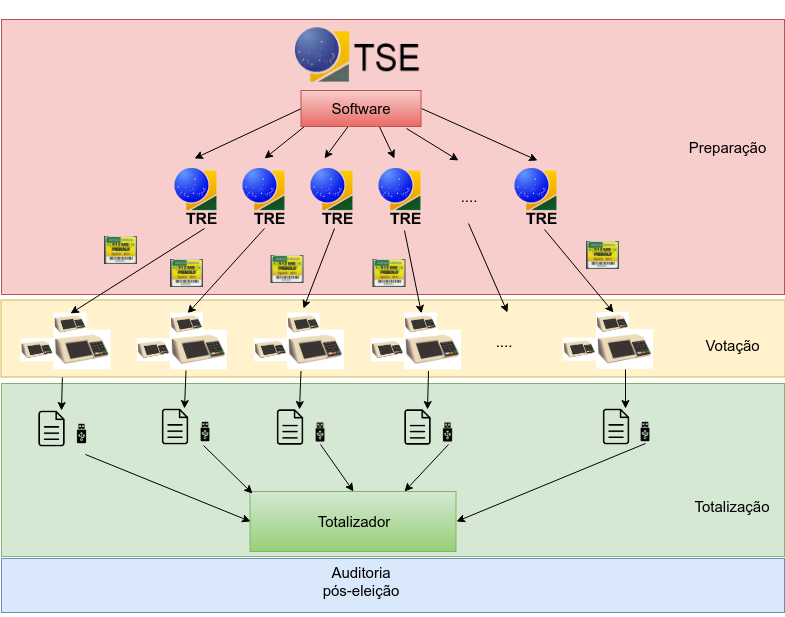
\includegraphics[width=\textwidth]{TSE.png}
\end{frame}


\begin{frame}{Preparação}
\begin{minipage}{0.75\textwidth}
\begin{enumerate}
 \item Confecção do \emph{software} de votação no TSE
 \item Transmissão do \emph{software} de votação para TREs
 \item Gravação do \emph{software} de votação em cartões de memória \emph{flash}
 \item Distribuição dos cartões de memória
 \item Instalação nas urnas eletrônicas (carga)
\end{enumerate}
\end{minipage}
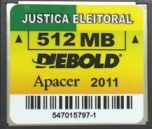
\includegraphics[scale=0.45]{flash.jpg}

\bigskip

\begin{flushright}
\begin{minipage}{.75\textwidth}
\begin{block}{\alert{Transparência}}\medskip
\begin{itemize}
 \item Exame por fiscais de partido, OAB, MPU, SBC
 \item Testes Públicos de Segurança
\end{itemize}
\end{block}
\end{minipage}
\end{flushright}
\end{frame}

\begin{frame}{Votação}
\begin{enumerate}
 \item Impressão da zerésima
 \item Sessão de votação (identificação biométrica, interação com urna)
 \item Impressão do Boletim de Urna (BU)
 \item Gravação digital na Mídia de Resultados (MR) de BU eletrônico, Registro Digital do Voto (RDV), etc.
\end{enumerate}

\bigskip

\begin{flushright}
\begin{minipage}{.75\textwidth}
\begin{block}{\alert{Transparência}}\medskip
\begin{itemize}
 \item Zerésima
 \item Votação paralela
 \item Registro Digital do Voto?
\end{itemize}
\end{block}
\end{minipage}
\end{flushright}
\end{frame}

\begin{frame}{Totalização}
\begin{enumerate}
 \item Transmissão dos resultados parciais
 \item Combinação dos resultados parciais
 \item Divulgação do resultado final
 \item Publicação dos BUs eletrônicos
\end{enumerate}

\bigskip

\begin{flushright}
\begin{minipage}{.75\textwidth}
\begin{block}{\alert{Transparência}}\medskip
\begin{itemize}
 \item Conferência entre BUs físico e eletrônico
 \item Totalização paralela
\end{itemize}
\end{block}
\end{minipage}
\end{flushright}

\end{frame}

\section{Limitações de transparência:\\ o que pode dar errado?}

\begin{frame}{Limitações na preparação}

\begin{block}{\alert{Fiscalização}}
\begin{itemize}
 \item Complexidade do \emph{software} de votação ($> 10^6$ linhas)
 \item Falta de treinamento formal dos fiscais
 \item Filiação ou indicação partidária
 \item Termo de Confidencialidade
\end{itemize}
\end{block}

\begin{block}{\alert{Testes Públicos de Segurança}}
\begin{itemize}
 \item Formato burocrático (8 tipos de formulários)
 \item Escopo e duração dos testes
 \item Condições de trabalho poucos realistas, não modelam atacante hábil
 \item Conflito de interesse intrínseco
 \item Termo de Confidencialidade (em 2016)
\end{itemize}
\end{block}
 
\end{frame}

\begin{frame}[fragile]{Limitações na votação}

\begin{block}{\alert{Zerésima e Votação paralela}}
\begin{itemize}
 \item Não previnem \emph{software} desonesto
 \item Simulação $\times$ Realidade (caso da Volkswagen)
 \item Tamanho e qualidade da amostra
\end{itemize}
\end{block}

\pause
Exemplo de comportamento nunca detectado na votação paralela:
\begin{verbatim}
    If (voto == 99999) {
        ativar_comportamento_malicioso();
    }
\end{verbatim}

\alert{Importante:} Assumir versão ofuscada escondida na base de código!
\end{frame}

\begin{frame}[fragile]{Limitações na totalização}

\begin{block}{\alert{Conferência}}
\begin{itemize}
 \item Limitação na emissão de BUs impressos
 \item Restrições logísticas (custo e cobertura)
 \item \emph{Projeto Você Fiscal} (2014 e 2016)
 \item Tamanho e qualidade da amostra
\end{itemize}
\end{block}

\alert{Importante:} É provavelmente a fase mais transparente do processo eleitoral eletrônico, especialmente após introdução do código QR.

\begin{flushright}
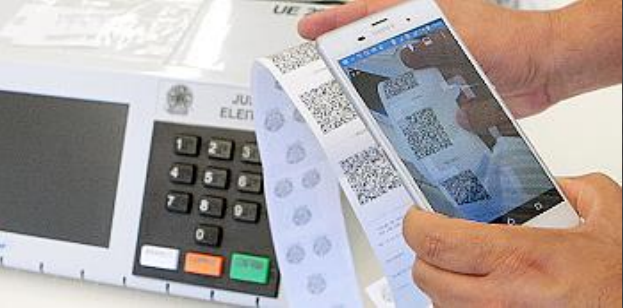
\includegraphics[width=0.5\textwidth]{qrcode.png}
\end{flushright}

\end{frame}

\begin{frame}{E uma auditoria pós-eleição?}
\begin{itemize}
\item Primeira realizada em 2014, relatório inconclusivo (``\emph{não permite a plena auditagem}'')
\item Meses para entrega de todos os arquivos e documentos
\item Conflito de interesse com o TSE e interesses partidiários
\item Influência da situação política
\end{itemize}

\bigskip

\begin{block}{Imprensa e audiência do TSE}
``\emph{Auditoria conclui que não houve fraude na eleição de 2014}''
\end{block}

\bigskip

\alert{Conclusão:} Sistema brasileiro eletrônico de votação {\bf não é auditável}.
\end{frame}

\section{Mas o \emph{software} é 100\% seguro!\\Somos líder em tecnologia eleitoral... certo?}

\begin{frame}
\begin{center}

\includegraphics[width=0.75\textwidth]{impossibru.png}
\end{center}
\end{frame}

\begin{frame}
\begin{center}

\includegraphics[width=\textwidth]{sextosentido.jpg}
\end{center}
\end{frame}

\begin{frame}{TPS 2012 -- Falhas descobertas}

\begin{itemize}
\item Vulnerabilidade trivial no {\bf sigilo do voto}
\item Compartilhamento e armazenamento inseguro de {\bf segredos} criptográficos
\item Verificação {\bf insuficiente} de integridade
\item Processo de desenvolvimento {\bf inseguro}
\item Modelo adversarial {\bf inadequado}
\item Cultura interna {\bf sem transparência}
\end{itemize}

\bigskip
\alert{Conclusão}: falhas graves tecnológicas e procedimentais!
\end{frame}

\begin{frame}{TPS 2012 -- Registro Digital do Voto}
\begin{center}
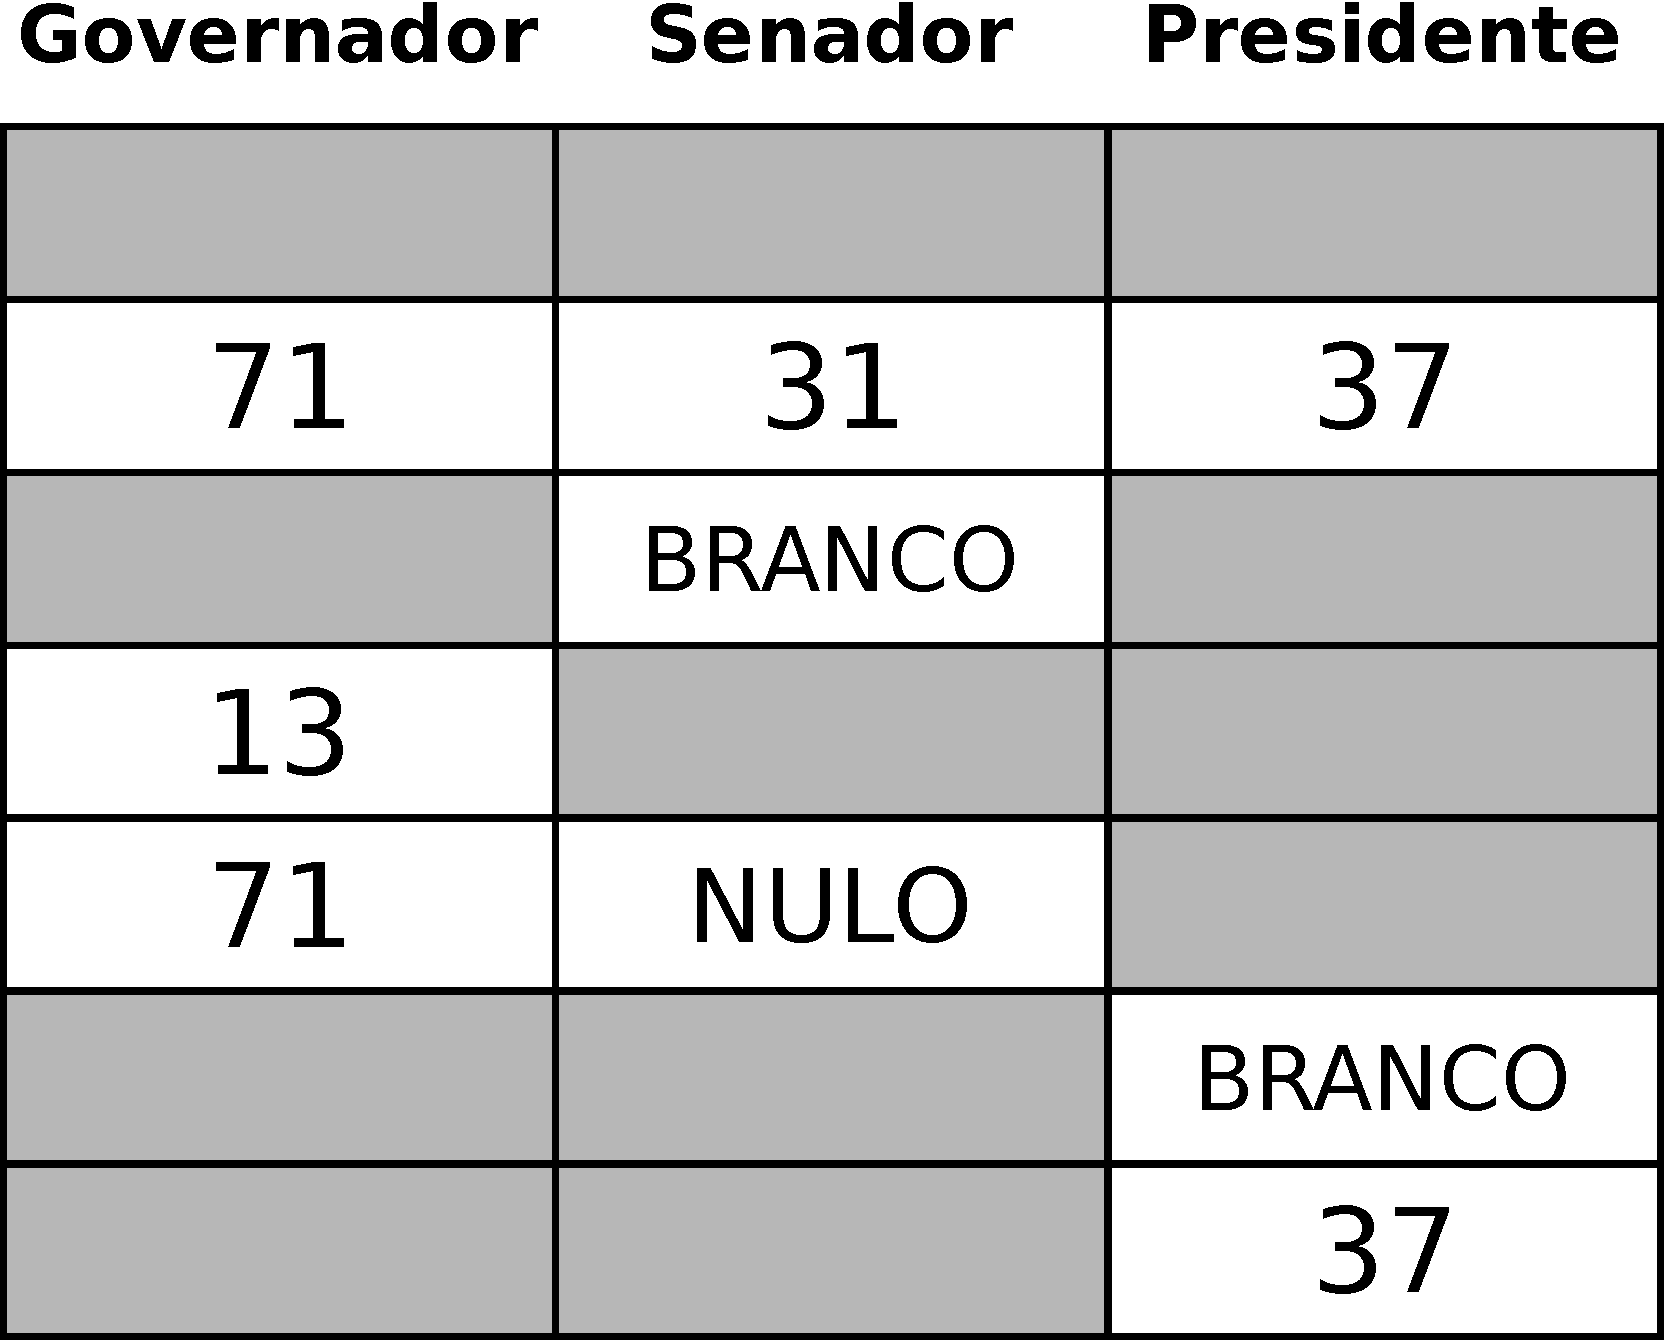
\includegraphics[scale=0.35]{rdv4.pdf}
\end{center}
\end{frame}

\begin{frame}{TPS 2012 -- Quebra do sigilo do voto}
\begin{center}
Semente \textbf{secreta e aleatória} para embaralhar RDV: \texttt{srand(time(NULL))}

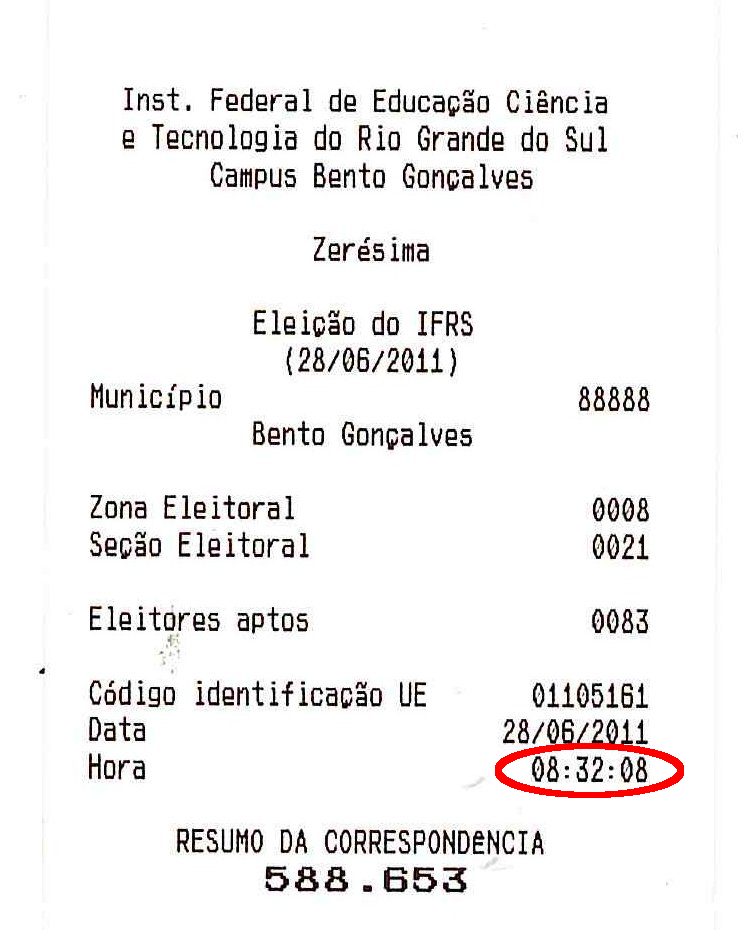
\includegraphics[width=0.5\textwidth]{semente.png}
\end{center}
\end{frame}

\begin{frame}[fragile]{TPS 2012 -- Defesa em profundidade?}
\begin{table}
 \begin{tabular}{cc}
\begin{minipage}{5cm}
\begin{verbatim}
File 1/1: lew.jpg
File name: lew.jpg
File size: 47009 Bytes
MIME type: image/jpeg
Image size: 276 x 360
Camera make: Canon
Camera model: Canon EOS-1Ds Mark III
Image timestamp: 2010:10:03 11:20:37
\end{verbatim}
\end{minipage} &
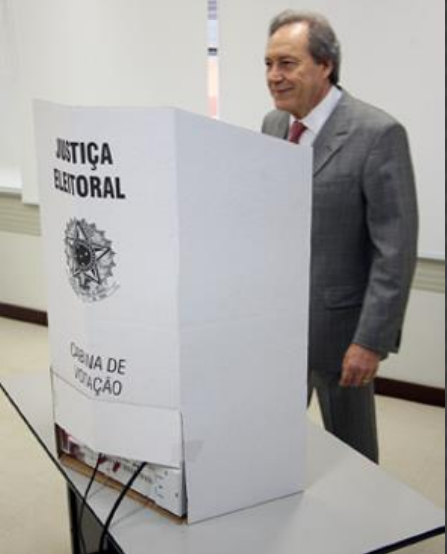
\includegraphics[scale=0.4]{lew.jpg}
 \end{tabular}
\end{table}
\end{frame}

\begin{frame}[fragile]{TPS 2016 -- Integridade do voto}
\begin{center}
Código de autenticação de BU para \textbf{digitação manual}:

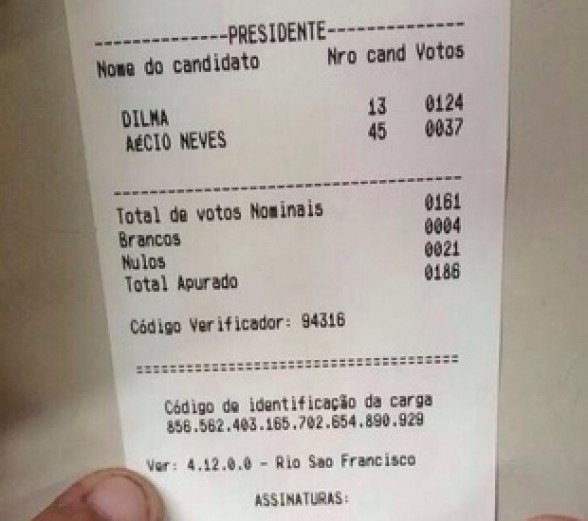
\includegraphics[width=0.7\textwidth]{bu.jpg}
\end{center}
\end{frame}

\begin{frame}{TPS 2017 -- Composição da equipe}

Montada pelo time \emph{ELT}, que participa de competições nacionais e internacionais de \emph{Capture The Flag} (CTF). Muitas das habilidades são equivalentes (curiosidade, ferramental, raciocínio adversarial):
\begin{itemize}
 \item Pedro: \emph{Assembly} e criptografia
 \item Thiago: \emph{Web} e exploração 
 \item Caio: Tecnologias \emph{Web}
 \item Paulo: Engenharia Reversa e exploração
 \item Diego: ecossistema da urna, formato dos testes, criptografia
\end{itemize}

\alert{Diversidade:} Todos os membros contribuíram com uma idéia fundamental em certo ponto que permitiu o avanço da equipe.
\end{frame}

\begin{frame}[fragile]{TPS 2017 -- Inspeção de código}

Edital de abertura especificava que investigadores não teriam acesso a chaves criptográficas.

\bigskip

\begin{block}{Interpretação do TSE}
Apagar as chaves criptográficas do código, ``\emph{para aumentar o desafio}''!
\end{block}

\bigskip
\pause

\alert{Falha operacional:} Felizmente, não apagaram todas. Encontramos chave em claro na versão 3.18 do \emph{kernel}. :)

\bigskip

Equipe fez uma análise inicialmente superficial do sistema, depois aprofundada nos {\bf mecanismos criptográficos}, que concentram \textbf{risco}.

\end{frame}

\begin{frame}{TPS 2017 -- Superfície de ataque}

Submetemos vários planos de teste, todos \textbf{aprovados}:
\begin{itemize}
 \item \emph{Captura de chaves criptográficas do \emph{flash} de carga}
 \item \emph{Execução remota de código na plataforma web}
 \item \emph{Tentativa de violação do sigilo do voto}
 \item \emph{Inserção de dispositivo USB malicioso}
\end{itemize}

Pela restrição de tempo, nos concentramos no primeiro ataque e suas consequências.

\end{frame}

\begin{frame}{TPS 2017 -- Ambiente}
\begin{center}
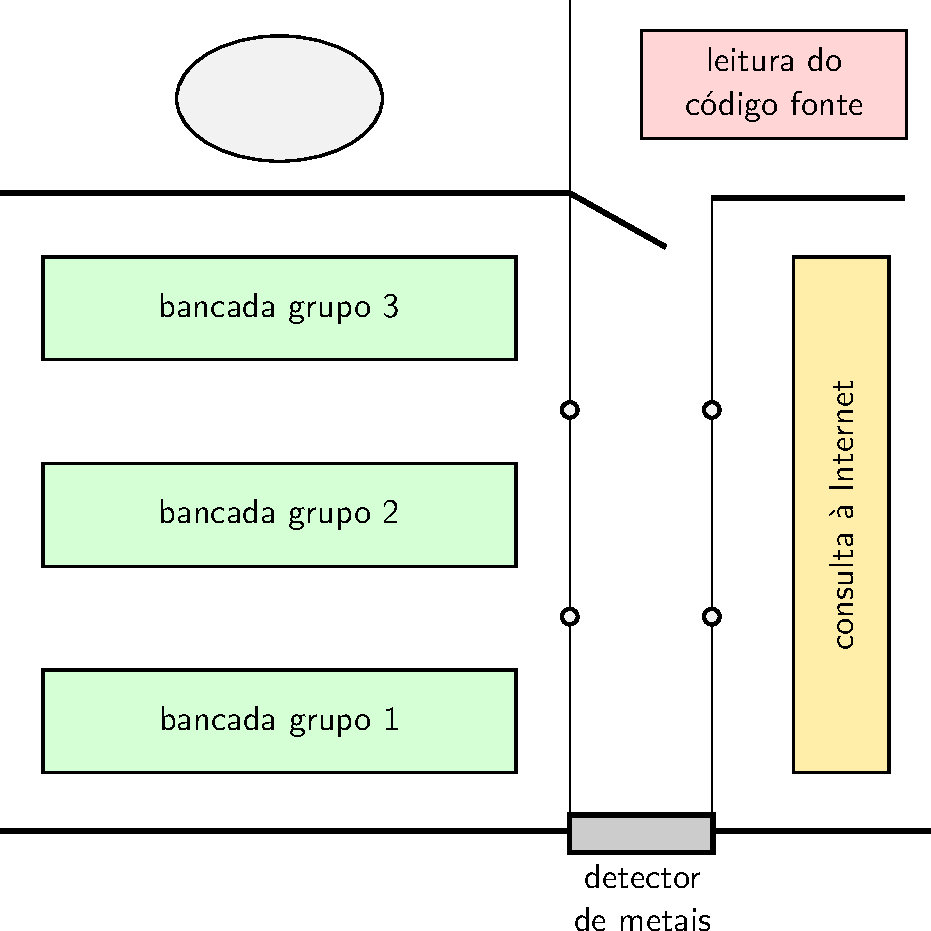
\includegraphics[scale=0.5]{planta.pdf}
\end{center}
\end{frame}


\begin{frame}{TPS 2017 -- Dia 1}

Praticamente dedicado a {\bf preencher formulários}, reconhecer o ambiente, solicitar computadores e começar a instalar Kali Linux nas máquinas.

\medskip

Os cartões de memória da urna eletrônica são cifrados com AES-256 em modo XTS, que exige duas chaves criptográficas, compartilhadas entre {\bf todas as urnas}.

\medskip

\alert{Progresso:} Descobrimos durante a inspeção de código uma {\bf presente no código-fonte} e a outra armazenada {\bf às claras} no cartão de memória.

\medskip

\alert{$\rightarrow$} \emph{Script} Python+OpenSSL em máquina de inspeção de código para decifrar um \emph{stub} da partição cifrada que encontramos por lá.

\end{frame}

\begin{comment}
\begin{frame}{TPS 2017 -- Dia 1}
 
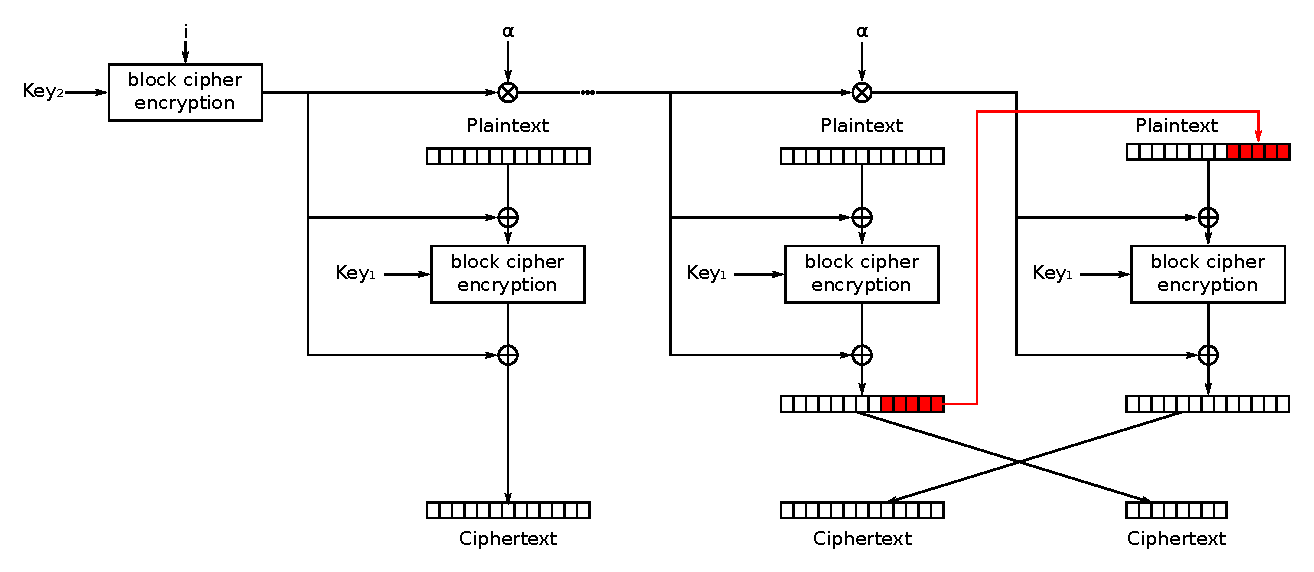
\includegraphics[width=\textwidth]{XTS_mode_encryption.pdf}

\alert{Importante:} IV foi escolhido como \emph{inode}, período de $\alpha^j$ recomeça após 256 blocos, $key_1$ estava no código-fonte, $key_2$ armazenado às claras no cartão de memória.

\end{frame}
\end{comment}

\begin{frame}{TPS 2017 -- Dia 2}

\alert{$\rightarrow$} Reimplementamos decifração de cartões de memória com \texttt{pycrypto} nas máquinas de teste, copiando a chave criptográfica {\bf memorizada} alguns \emph{bytes} por vez.

\bigskip

Após decifrar o cartão inteiro, estudamos a verificação de integridade:

\begin{center}
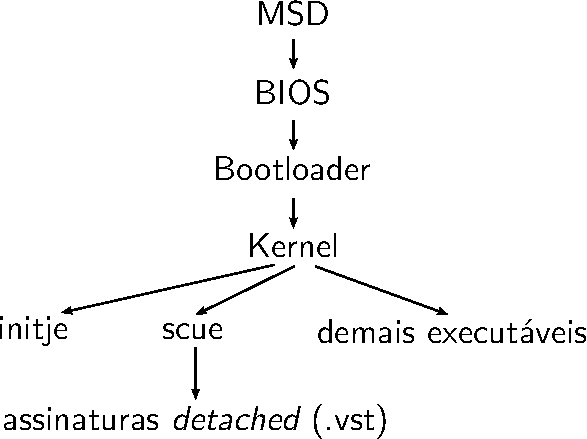
\includegraphics[scale=0.5]{autenticacao.pdf}
\end{center}

\alert{Problema:} Recebemos a visita de observadores internacionais, que atrapalharam bastante. :(

\end{frame}

\begin{frame}{TPS 2017 -- Dia 3}

\alert{Progresso:} Encontramos duas bibliotecas (\texttt{libapilog.so} e \texttt{libhkdf.so}) {\bf sem assinaturas digitais}.

\bigskip

\alert{$\rightarrow$} Injetamos trechos de código simples nessas bibliotecas para verificar se versões adulteradas eram devidamente instaladas na carga.

\bigskip

\alert{$\rightarrow$} Alteramos todas as chamadas de uma das bibliotecas para imprimir \texttt{FRAUDE!} no terminal, o que aconteceu. :)

\end{frame}

\begin{frame}{TPS 2017 -- Dia 4}

Exploramos ataques contra o sistema utilizando as funcionalidades fornecidas pelas bibliotecas:
\begin{itemize}
 \item \texttt{libapilog.so}: conseguimos adulterar o registro de \emph{log} substituindo \texttt{INFO} por \texttt{XXXX}.
 \item \texttt{libhkdf.so}: conseguimos adulterar a biblioteca para zerar chave criptográfica derivada para cifrar RDV.
\end{itemize}

\alert{$\rightarrow$} Implementamos ainda um programa para receber e imprimir comandos de um teclado {\bf acoplado à urna}. :)

\medskip

\alert{Progresso:} Cifrar o RDV com uma chave conhecida permite \textbf{violar sigilo de um voto específico}.

\end{frame}

\begin{frame}{TPS 2017 -- Dia 5}

Após conseguir desempacotar o programa de votação \texttt{vota} com UPX, percebemos que estava ligado com as duas bibliotecas.

\bigskip

\alert{Progresso:} Injetamos código para alterar a versão do \emph{software} e o {\bf conteúdo da tela} em tempo de execução:

\bigskip

\alert{$\rightarrow$} Passamos as últimas horas trabalhando em interferir com a contagem de votos, e chegamos a produzir \textbf{erro de consistência por cédula vazia}.

\bigskip

\alert{Observação:} Conseguimos controle sobre o software de votação para {\bf injeção de código arbitrário}.

\bigskip

\alert{Problema:} Tivemos que preparar uma demonstração dos resultados parciais, o que tomou mais tempo. :(

\end{frame}

\begin{frame}{TPS 2017 -- Dia 5}

\alert{Progresso:} Peritos da Polícia Federal {\bf recuperam} a chave de cifração diretamente do \emph{bootloader}, mostrando que acesso a código-fonte {\bf não é obrigatório}.

\begin{center}
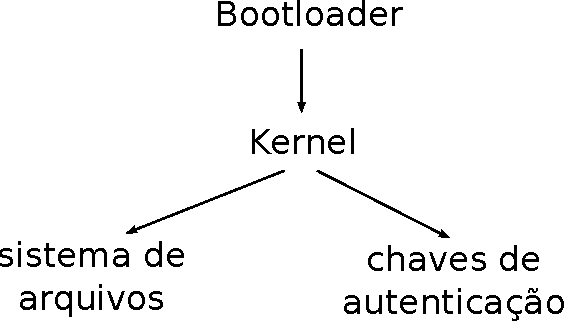
\includegraphics[scale=0.5]{cifracao.pdf}
\end{center}

\alert{Observação:} acesso a uma única chave de encriptação fornece {\bf poder desproporcional} a um atacante. {\bf Sempre questionar premissas!}

\end{frame}

\begin{comment}
\begin{frame}{TPS 2017 -- Dia 5}

\begin{center}
\animategraphics[loop,width=0.9\linewidth]{24}{images/cropped-}{0}{300}
\end{center}

\end{frame}
\end{comment}

\begin{frame}{TPS 2017 -- Resultado principal}

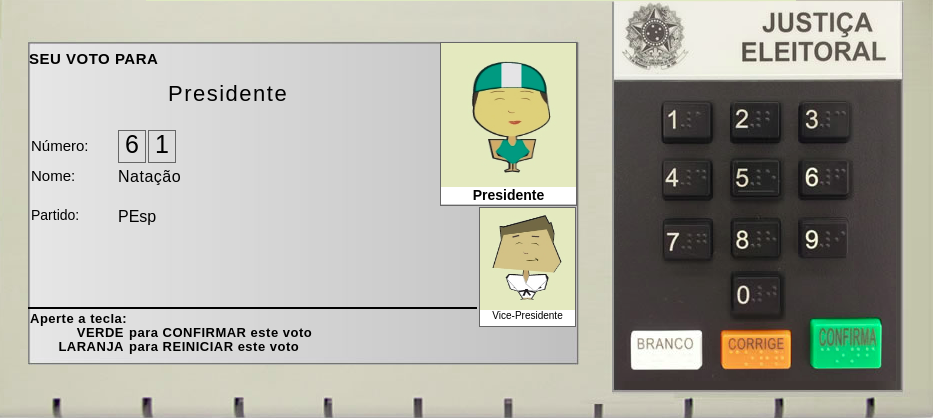
\includegraphics[width=\textwidth]{tela-original.png}

\end{frame}

\begin{frame}{TPS 2017 -- Resultado principal}

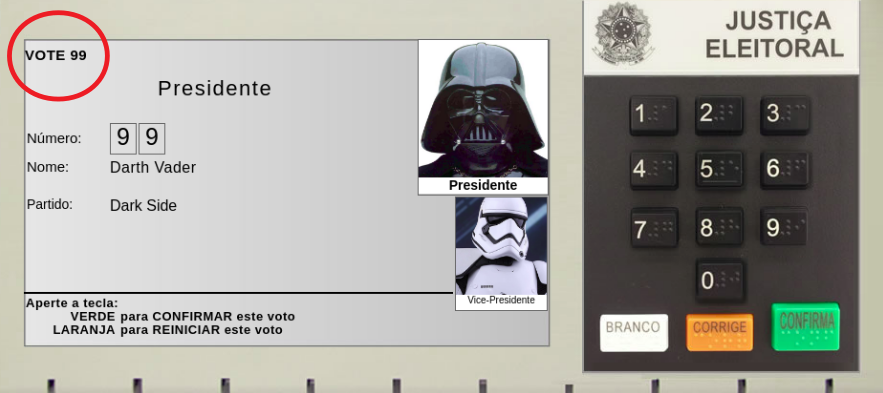
\includegraphics[width=\textwidth]{tela-adulterada.png}

\end{frame}

\begin{frame}{Solução independente de \emph{software}}
\begin{figure}
\caption{Máquina de votar utilizada no México com trilha de auditoria em papel (VVPAT)}
\begin{center}
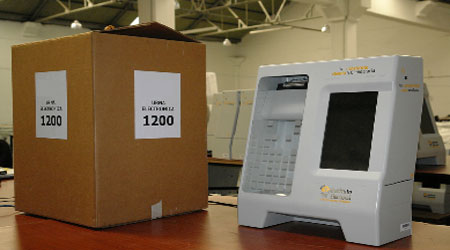
\includegraphics[scale=0.6]{mexico.jpg} 
\end{center}
\end{figure}
\end{frame}

\begin{frame}{Solução independente de \emph{software}}
\begin{figure}
\caption{Máquina de votar utilizada na Índia com trilha de auditoria em papel (VVPAT)}
\begin{center}
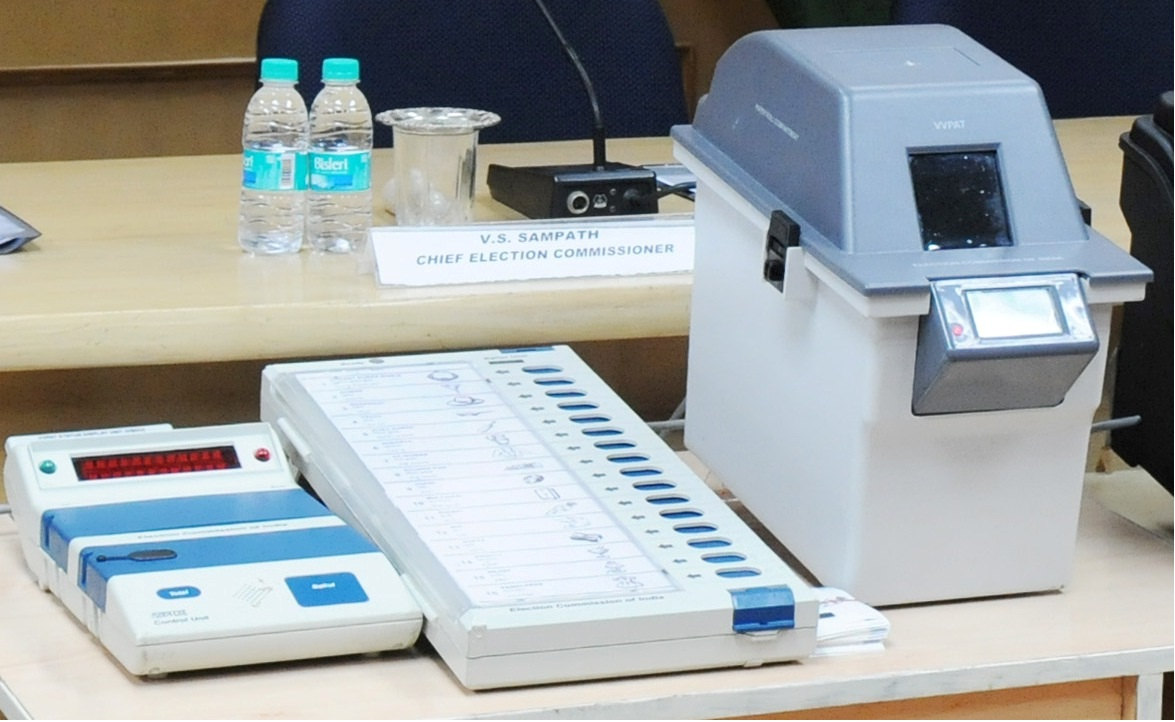
\includegraphics[scale=0.35]{india.jpg} 
\end{center}
\end{figure}
\end{frame}

\begin{frame}{Solução independente de \emph{software}}
\begin{figure}
\caption{Máquina de votar utilizada na Venezuela com trilha de auditoria em papel (VVPAT)}
\begin{center}
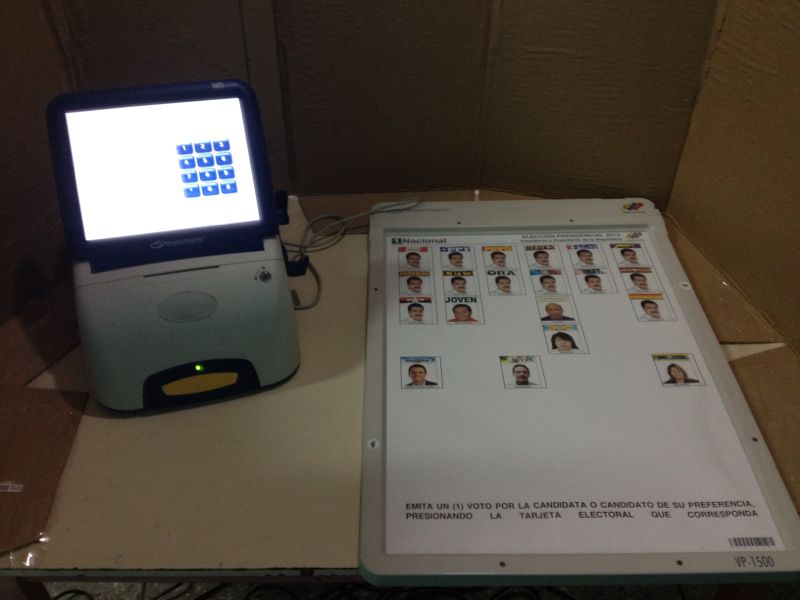
\includegraphics[scale=0.35]{venezuela.jpg} 
\end{center}
\end{figure}
\end{frame}

\begin{frame}{Solução independente de \emph{software}}
\begin{figure}
\caption{Sistema de votação utilizado na Argentina (E2E?).}
\begin{center}
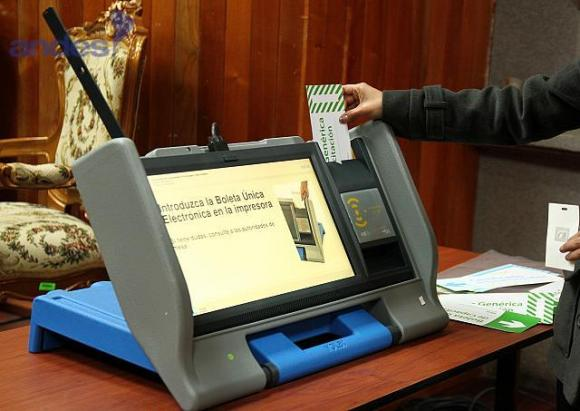
\includegraphics[scale=0.4]{argentina.jpg} 
\end{center}
\end{figure}
\end{frame}


\begin{frame}{Solução independente de \emph{software}}
\begin{figure}
\caption{Máquinas utilizadas nos Estados Unidos como scanners de votos.}
\begin{center}
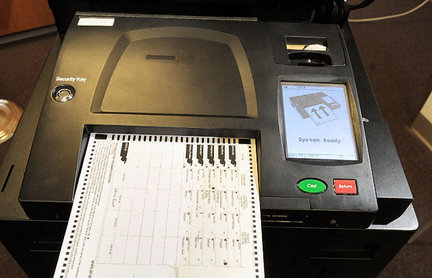
\includegraphics[scale=0.4]{scanner.jpg} 
\end{center}
\end{figure}
\end{frame}

\begin{frame}{Conclusões}

Violadas ao menos duas barreiras de segurança:
\begin{itemize}
 \item \emph{Cifração das mídias} (erro de projeto)
 \item \emph{Autenticação de bibliotecas compartilhadas} (falha procedimental e erro de projeto)
\end{itemize}

\alert{Crítico:} Projeto depende fundamentalmente da ofuscação do \emph{bootloader} para impedir ataques.

\medskip
Observações adicionais:
\begin{itemize}
 \item Tempo dos testes \textbf{não é comparável} a ataque real;
 \item Não é factível seguir \textbf{estritamente} o protocolo formal dos testes, usamos muitos atalhos.
\end{itemize}
\end{frame}

\begin{frame}{Problemas...}
\begin{block}{... que persistem:}
\begin{enumerate}
\item \emph{Software} {\bf secreto} por mais de 20 anos
\item \emph{Software} {\bf demonstravelmente} inseguro em múltiplas ocasiões
\item Ausência de {\bf recontagem}
\item Ausência de auditoria {\bf efetiva}
\item {\bf Conflitos de interesse} em todo lugar
\item {\bf Ataques internos} completamente ignorados
\end{enumerate}
\end{block}
\end{frame}

\begin{frame}{O que fazer?}
\begin{block}{1. Voto impresso}
\it Implementar registro físico e anônimo do voto, conferível pelo eleitor, para auditoria/recontagem. 
\end{block}

\bigskip

\begin{block}{2. Código aberto}
\it Publicar código-fonte do \emph{software} é desejável para ampliar a capacidade de auditoria, mas insuficiente. Favor não esquecer de mover chaves criptográficas para lugar seguro. :)
\end{block}

\bigskip

\begin{block}{3. Controle social}
\it Ampliar mecanismos de transparência para que sociedade possa exercer maior controle social sobre o sistema, financiado por recursos públicos.
\end{block}
\end{frame}

\begin{frame}[standout]
\begin{center}
{\LARGE \alert{Perguntas?}}\\\
{\bf D. F. Aranha}\\
\texttt{dfaranha@ic.unicamp.br}\\
\texttt{@dfaranha}
\end{center}
\end{frame}

\begin{frame}{Referências}

\begin{enumerate}
 \item Diego F. Aranha, Marcelo M. Karam, André de Miranda, Felipe Scarel.
 \textbf{Software vulnerabilities in the Brazilian voting machine}.
In: \emph{Design, Development, and Use of Secure Electronic Voting Systems}, 149-175, IGI Global, 2014.
\item Diego F. Aranha, Helder Ribeiro, André Luiz Ogando Paraense.
\textbf{Crowdsourced integrity verification of election results: an experience from Brazilian elections}.
Annals of Telecommunications, 71(7), 287-297, 2016.
\item Diego F. Aranha, Pedro Y. S. Barbosa, Thiago N. C. Cardoso, Caio Lüders de Araújo, Paulo Matias. \textbf{The Return of Software Vulnerabilities in the Brazilian Voting Machine}, Relatório Técnico, 2018.
\end{enumerate}


\end{frame}


\end{document}
